\documentclass[12pt,fleqn]{article}

%%%%%%%%%%%%%%%%%%%%%%%%%%%%%%%%%%%%%%%%%%%%%%%%%%%%%%%%%%%%%%%%%%%%%
% CONFIGURAÇÃO DE IDIOMA E CODIFICAÇÃO
%%%%%%%%%%%%%%%%%%%%%%%%%%%%%%%%%%%%%%%%%%%%%%%%%%%%%%%%%%%%%%%%%%%%%

\usepackage[utf8]{inputenc}   % Codificação UTF-8
\usepackage[T1]{fontenc}      % Codificação de fontes
%\usepackage[brazil]{babel}    % Português do Brasil (Babel moderno)

%%%%%%%%%%%%%%%%%%%%%%%%%%%%%%%%%%%%%%%%%%%%%%%%%%%%%%%%%%%%%%%%%%%%%
% PACOTES DO TEMPLATE
%%%%%%%%%%%%%%%%%%%%%%%%%%%%%%%%%%%%%%%%%%%%%%%%%%%%%%%%%%%%%%%%%%%%%

\usepackage{setup/config}     % Arquivo de estilo do evento
\usepackage{natbib}           % Sistema de citações
\usepackage{graphicx}         % Inserção de figuras
\usepackage{color}            % Controle de cores
\usepackage{wallpaper}        % Imagens de fundo
\usepackage{hyperref}         % Links e referências
\usepackage{titlesec}         % Controle de títulos
\usepackage{float}            % Permite usar [H] em figuras/tabelas
\usepackage{fancyhdr}         % Cabeçalhos e rodapés

%%%%%%%%%%%%%%%%%%%%%%%%%%%%%%%%%%%%%%%%%%%%%%%%%%%%%%%%%%%%%%%%%%%%%
% DIRETÓRIO DAS FIGURAS
%%%%%%%%%%%%%%%%%%%%%%%%%%%%%%%%%%%%%%%%%%%%%%%%%%%%%%%%%%%%%%%%%%%%%

\graphicspath{{figures/}}

%%%%%%%%%%%%%%%%%%%%%%%%%%%%%%%%%%%%%%%%%%%%%%%%%%%%%%%%%%%%%%%%%%%%%
% AJUSTE DE ESPAÇAMENTO NA BIBLIOGRAFIA
%%%%%%%%%%%%%%%%%%%%%%%%%%%%%%%%%%%%%%%%%%%%%%%%%%%%%%%%%%%%%%%%%%%%%

% Reduz espaçamento entre referências
\let\OLDthebibliography\thebibliography
\renewcommand\thebibliography[1]{%
\OLDthebibliography{#1}
\setlength{\parskip}{0pt}
\setlength{\itemsep}{0pt plus 0.3ex}
}

%%%%%%%%%%%%%%%%%%%%%%%%%%%%%%%%%%%%%%%%%%%%%%%%%%%%%%%%%%%%%%%%%%%%%
% TÍTULO DO ARTIGO
%%%%%%%%%%%%%%%%%%%%%%%%%%%%%%%%%%%%%%%%%%%%%%%%%%%%%%%%%%%%%%%%%%%%%

\title{BIOSENSIA-DC: A DRUGCLIP-BASED COMPUTATIONAL PROTOTYPE FOR TARGET FISHING APPLIED TO BIORECEPTOR DISCOVERY}

%%%%%%%%%%%%%%%%%%%%%%%%%%%%%%%%%%%%%%%%%%%%%%%%%%%%%%%%%%%%%%%%%%%%%
% AUTORES E AFILIAÇÕES
%%%%%%%%%%%%%%%%%%%%%%%%%%%%%%%%%%%%%%%%%%%%%%%%%%%%%%%%%%%%%%%%%%%%%

\author{
\rm
\begin{tabular}{l}
\textbf{First Author}$^{1}$ - {\textnormal e-mail}\\
\textbf{Second Author}$^{2}$ - {\textnormal e-mail}\\
\textbf{Third Author}$^{3}$ - {\textnormal e-mail}\\
{\fontsize{11}{0}\selectfont $^{1}$Universidade Federal do Rio Grande – Rio Grande – RS}\\
{\fontsize{11}{0}\selectfont $^{2}$Universidade Federal do Rio Grande – Santo Antônio da Patrulha – RS}\\
{\fontsize{11}{0}\selectfont $^{3}$Universidade Federal do Rio Grande – São Lourenço do Sul – RS}
\end{tabular}
}

%%%%%%%%%%%%%%%%%%%%%%%%%%%%%%%%%%%%%%%%%%%%%%%%%%%%%%%%%%%%%%%%%%%%%
% RODAPÉ ESPECIAL DA PRIMEIRA PÁGINA
%%%%%%%%%%%%%%%%%%%%%%%%%%%%%%%%%%%%%%%%%%%%%%%%%%%%%%%%%%%%%%%%%%%%%

\fancypagestyle{firstpagestyle}
{
\renewcommand{\headrulewidth}{0pt}

\fancyfoot[C]{
\footnotesize
\parbox{15cm}{
\centering
\fontsize{7.5}{0}\selectfont\it
XXIX ENMC – Encontro Nacional de Modelagem Computacional\\
XVII ECTM – Encontro de Ciência e Tecnologia de Materiais\\
06 a 09 de outubro de 2026 - Bento Gonçalves - RS
}}
}


%%%%%%%%%%%%%%%%%%%%%%%%%%%%%%%%%%%%%%%%%%%%%%%%%%%%%%%%%%%%%%%%%%%%%
% PACOTES
%%%%%%%%%%%%%%%%%%%%%%%%%%%%%%%%%%%%%%%%%%%%%%%%%%%%%%%%%%%%%%%%%%%%%

\usepackage{tikz}
\usetikzlibrary{arrows.meta, positioning, calc}

%%%%%%%%%%%%%%%%%%%%%%%%%%%%%%%%%%%%%%%%%%%%%%%%%%%%%%%%%%%%%%%%%%%%% 
% INÍCIO DO DOCUMENTO
%%%%%%%%%%%%%%%%%%%%%%%%%%%%%%%%%%%%%%%%%%%%%%%%%%%%%%%%%%%%%%%%%%%%%

\begin{document}

\pretolerance=10000

%%%%%%%%%%%%%%%%%%%%%%%%%%%%%%%%%%%%%%%%%%%%%%%%%%%%%%%%%%%%%%%%%%%%%
% LOGO DO EVENTO
%%%%%%%%%%%%%%%%%%%%%%%%%%%%%%%%%%%%%%%%%%%%%%%%%%%%%%%%%%%%%%%%%%%%%

\begin{figure}
\centering

\includegraphics[width=6.25in]{logo.png}
\end{figure}

\vspace{-3cm}

%%%%%%%%%%%%%%%%%%%%%%%%%%%%%%%%%%%%%%%%%%%%%%%%%%%%%%%%%%%%%%%%%%%%%
% TÍTULO
%%%%%%%%%%%%%%%%%%%%%%%%%%%%%%%%%%%%%%%%%%%%%%%%%%%%%%%%%%%%%%%%%%%%%

\maketitle

\pagestyle{empty}
\thispagestyle{firstpagestyle}

%%%%%%%%%%%%%%%%%%%%%%%%%%%%%%%%%%%%%%%%%%%%%%%%%%%%%%%%%%%%%%%%%%%%%
% RESUMO
%%%%%%%%%%%%%%%%%%%%%%%%%%%%%%%%%%%%%%%%%%%%%%%%%%%%%%%%%%%%%%%%%%%%%

\begin{abstract}

  ???.
  
% To be written after the main text.
% Suggested content:

% - Introduce BioSensIA as a project aimed at supporting the discovery of biorecognition elements for biosensors.

% - Present BioSensIA-DC as a computational prototype for target fishing: given a query molecule, rank candidate protein pockets.

% - Explain that the prototype adapts DrugCLIP, originally designed for virtual screening, to the reverse direction: molecule-to-pocket retrieval.

% - Highlight implementation contributions: construction of candidate-pocket LMDB files, query-molecule LMDB files, molecule lookup via SMILES/PubChem, target-fishing retrieval, and an initial benchmarking workflow.

% - State clearly that the current quantitative results are preliminary and unsatisfactory, including for the original DrugCLIP model in the local evaluation setup.

% - Frame the paper as a methodological and computational-prototype report, not as a validated performance claim.
  
\end{abstract}

\keywords{\em{Biosensors, Target fishing, DrugCLIP, Contrastive learning, Chemoinformatics}}

%%%%%%%%%%%%%%%%%%%%%%%%%%%%%%%%%%%%%%%%%%%%%%%%%%%%%%%%%%%%%%%%%%%%%
% CABEÇALHO DAS DEMAIS PÁGINAS
%%%%%%%%%%%%%%%%%%%%%%%%%%%%%%%%%%%%%%%%%%%%%%%%%%%%%%%%%%%%%%%%%%%%%

\fancyhead[L]{\footnotesize{\fontsize{7.5}{0}\selectfont\it
XXIX ENMC, XVII ECTM\\
06 a 09 de outubro de 2026}}

\renewcommand{\headrulewidth}{0pt}

\fancyfoot[C]{
\footnotesize
\parbox{15cm}{
\centering
\fontsize{7.5}{0}\selectfont\it
XXIX ENMC – Encontro Nacional de Modelagem Computacional\\
XVII ECTM – Encontro de Ciência e Tecnologia de Materiais\\
06 a 09 de outubro de 2026 - Bento Gonçalves - RS
}}

\rhead{}

\pagestyle{fancy}

%%%%%%%%%%%%%%%%%%%%%%%%%%%%%%%%%%%%%%%%%%%%%%%%%%%%%%%%%%%%%%%%%%%%%
% INÍCIO DO TEXTO
%%%%%%%%%%%%%%%%%%%%%%%%%%%%%%%%%%%%%%%%%%%%%%%%%%%%%%%%%%%%%%%%%%%%%


\section{INTRODUCTION}

\subsection{Biosensors and the bioreceptor-selection problem}

A biosensor can be understood as an analytical device that couples a
biological recognition mechanism to a signal-transduction mechanism.
The biological component is responsible for interacting with the
analyte of interest, while the transducer converts that interaction
into a measurable signal. In this work, we use the terms
\emph{bioreceptor} and \emph{biorecognition element} in this general
sense. Common examples include enzymes, antibodies, aptamers,
receptors, and other biomolecular structures capable of selective
molecular recognition
\citep{eggins96:_biosen,banica12:_chemic_sensor_biosen,morales18:_guide_selec_biorec_elemen_biosen}.
The nature of this recognition element strongly influences the
sensitivity, selectivity, reproducibility, and practical applicability
of the resulting biosensor.

Selecting a suitable bioreceptor is therefore one of the central
design decisions in biosensor development. This decision is not merely
a matter of choosing a molecule that can bind the analyte: the
candidate must also be compatible with immobilization, signal
generation, stability requirements, sample conditions, and the
intended sensing platform. Enzyme-based biosensors, immunosensors, and
aptamer-based sensors offer different advantages and limitations, but
each case still requires the identification of a recognition mechanism
that is selective enough for the target application
\citep{marques08:_bioss,morales18:_guide_selec_biorec_elemen_biosen}.

The broader BioSensIA project addresses this problem as a
computational discovery task. Given an analyte molecule, the goal is
to identify proteins, protein domains, binding pockets, or other
biomolecular structures that may interact with it and therefore
deserve further investigation as candidate bioreceptors. In this
formulation, the computational system is not expected to replace
experimental validation. Rather, it is intended to reduce the search
space: instead of manually inspecting many unrelated biological
databases and structural records, the user receives a prioritized list
of candidates that can be examined with additional structural,
biochemical, and bibliographic evidence. This ranking-oriented view is
particularly useful when the biological interactions relevant to
sensing are not already obvious from the literature.

BioSensIA-DC is one computational component of this broader workflow.
It focuses on the structural target-fishing step: given a query
molecule, it ranks candidate protein pockets according to a learned
compatibility score. The prototype is based on DrugCLIP, a contrastive
representation-learning model originally proposed for virtual
screening, and on Uni-Mol-style three-dimensional molecular and pocket
representations \citep{gao23:_drugc,zhou23:_uni_mol}. BioSensIA-DC
uses DrugCLIP as a representation-learning foundation, but extends it
with a new target-fishing workflow, data organization strategy, and
retrieval implementation. In the original
virtual-screening direction, a protein pocket is used as a query to
rank molecules. BioSensIA-DC uses the same molecule--pocket
compatibility idea in the reverse direction: the molecule becomes the
query, and protein pockets become the candidates to be ranked. The
resulting ranked list is intended to support bioreceptor discovery,
not to provide a definitive proof of binding or biosensor performance.

\subsection{Virtual screening, target fishing, and representation learning}

Virtual screening and target fishing are closely related computational
tasks, but they differ in the direction of the query. In
structure-based virtual screening, the starting point is usually a
biological target, often represented by a protein binding pocket, and
the goal is to rank molecules from a candidate library according to
their predicted compatibility with that target. In target fishing, the
direction is reversed: the starting point is a molecule, and the goal
is to identify proteins, protein domains, binding sites, or other
biological targets that may interact with it. In both cases, the
practical output is a ranked list, but the biological interpretation
is different. Virtual screening asks which molecules may bind a given
target; target fishing asks which targets may bind a given molecule.

Several \emph{in silico} target-fishing strategies have been proposed,
including ligand-based, receptor-based, pharmacophore-based,
docking-based, and machine-learning approaches
\citep{galati21:_recen_advan_in_silic_target_fishin}. PharmMapper is a
representative example of reverse pharmacophore mapping. Given a query
compound, it searches for good alignments between the compound and a
database of pharmacophore models associated with protein targets
\citep{liu10:_pharm}. Its updated version expanded the target
pharmacophore database and introduced statistically meaningful ranking
scores for the identified targets \citep{wang17:_pharm}. In simplified
terms, PharmMapper asks whether the three-dimensional arrangement of
chemical features in the query molecule can be fitted to pharmacophore
patterns known or inferred for possible targets.

SwissTargetPrediction follows a different principle. It predicts
probable targets of a small molecule by comparing the query compound
to molecules with known bioactivity data. The method is based on the
similarity principle: molecules that are similar in two-dimensional or
three-dimensional chemical space are more likely to share biological
targets \citep{daina19:_swiss}. Thus, while PharmMapper is primarily
organized around reverse matching against pharmacophore models,
SwissTargetPrediction is organized around ligand similarity to
compounds with experimentally known target annotations. Both tools are
valuable references for BioSensIA because they address the same broad
question: given a molecule, which biological targets should be
considered plausible?

BioSensIA-DC differs from these tools in its representation-learning
formulation. Instead of matching a query molecule against an explicit
pharmacophore database, as in PharmMapper, or inferring targets from
similarity to known ligands, as in SwissTargetPrediction, \emph{BioSensIA-DC
uses a learned compatibility model between molecules and protein
pockets}. Its starting point is DrugCLIP, a contrastive learning model
that represents molecules and protein pockets with separate encoders
and trains them so that compatible molecule--pocket pairs are close in
a shared latent space \citep{gao23:_drugc}. DrugCLIP formulates
virtual screening as a dense-retrieval problem: a pocket is encoded as
a query vector, molecules are encoded as candidate vectors, and
ranking is performed by comparing these vectors.


The encoders used by DrugCLIP are based on Uni-Mol, a
three-dimensional molecular representation-learning framework that
incorporates atom types and atomic coordinates
\citep{zhou23:_uni_mol}. A key feature of Uni-Mol is that it is
designed to respect the geometry of molecular structures: its internal
pair representations are built from interatomic distances, which are
invariant to global translations and rotations of the molecule or
pocket. At the same time, Uni-Mol includes an equivariant
coordinate-prediction mechanism, so that when coordinates are
predicted or updated, they transform consistently under rotations and
translations of the input structure. In practical terms, this means
that the representation is sensitive to the relative three-dimensional
arrangement of atoms, but not to arbitrary choices of
coordinate-system origin or orientation. 

The central idea behind BioSensIA-DC is that the similarity score
learned by DrugCLIP can be used in the reverse direction. If DrugCLIP
can assign a compatibility score to a molecule--pocket pair for
virtual screening, then the same score can be used to rank pockets for
a fixed molecule. However, BioSensIA-DC is not merely a direct
execution of the original DrugCLIP workflow. DrugCLIP provides the
initial molecule--pocket representation framework, but the
target-fishing formulation, candidate-pocket preparation, query
construction, molecule-to-pocket retrieval pipeline, and initial
diagnostic evaluation workflow were conceptualized and implemented
from scratch as part of this work. The resulting prototype therefore
adapts a virtual-screening representation model to the
biosensor-oriented problem of prioritizing candidate bioreceptors for
a query analyte.

\subsection{Objectives and contributions}

This paper describes BioSensIA-DC, a computational prototype for
molecule-to-pocket target fishing in the context of bioreceptor
discovery. The prototype extends the DrugCLIP representation framework
beyond its original virtual-screening workflow. Instead of ranking
molecules for a fixed protein pocket, BioSensIA-DC ranks candidate
protein pockets for a fixed query molecule, producing a prioritized
list of structural candidates for further investigation.

The implemented contributions include the construction of
candidate-pocket files from DrugCLIP-compatible data, the construction
of query-molecule files from SMILES strings, local DrugCLIP
identifiers, PubChem CIDs, or compound names, and the implementation
of molecule-to-pocket retrieval. The prototype also generates ranked
pocket lists with compatibility scores, and provides an initial
benchmarking and diagnostic workflow.

The present work should be read as a computational-prototype and
methodology paper. Suitable benchmark validation has not yet been
completed. Therefore, no claim is made that the current model is
already a reliable target-fishing predictor. Instead, the paper
reports the implemented workflow, the conceptual adaptation from
virtual screening to target fishing, and the diagnostic issues that
must be resolved before predictive performance can be assessed.

\section{METHODOLOGY}

\subsection{Overview of the BioSensIA-DC workflow}

BioSensIA-DC implements a molecule-to-pocket retrieval workflow for
target fishing. The input is one or more query molecules, and the
output is a ranked list of candidate protein pockets. The workflow
reuses the molecule and pocket encoders from DrugCLIP, but reverses
the practical direction of retrieval: instead of using a pocket to
rank molecules, it uses a molecule to rank pockets.

The candidate protein pockets are stored in a library, which can be
encoded once and cached for later searches. During retrieval,
BioSensIA-DC encodes the query molecule, loads or computes the
candidate-pocket embeddings, calculates molecule--pocket similarity
scores, and sorts the candidate pockets by these scores.
Figure~\ref{fig:biosensia-dc-workflow} illustrates this workflow.

The resulting ranked list is saved for downstream analysis. Each entry
contains a candidate pocket identifier and a compatibility score. This
score is used only for ranking; it should not be interpreted as a
calibrated binding affinity or as a direct physical measurement.

\begin{figure}[htbp]
\centering
\resizebox{\linewidth}{!}{%
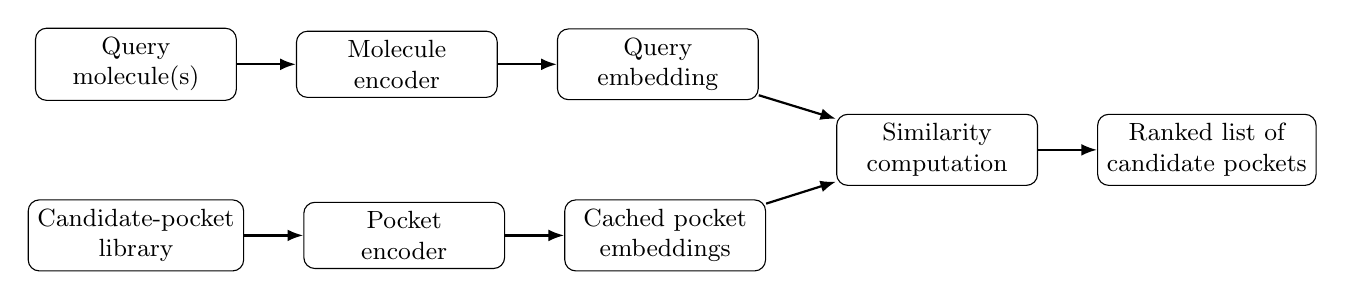
\begin{tikzpicture}[
  node distance=1.1cm and 0.75cm,
  box/.style={
    draw,
    rounded corners,
    align=center,
    minimum width=2.55cm,
    minimum height=0.82cm,
    font=\small
  },
  arrow/.style={-{Latex[length=2mm]}, thick}
]

% Molecule branch
\node[box] (molinput) {Query\\molecule(s)};
\node[box, right=of molinput] (molenc) {Molecule\\encoder};
\node[box, right=of molenc] (molemb) {Query\\embedding};

% Pocket branch
\node[box, below=1.25cm of molinput] (pocketlib) {Candidate-pocket\\library};
\node[box, right=of pocketlib] (pocketenc) {Pocket\\encoder};
\node[box, right=of pocketenc] (pocketemb) {Cached pocket\\embeddings};

% Shared scoring and output
\node[box] (sim) at ($(molemb)!0.5!(pocketemb)+(3.5cm,0)$)
  {Similarity\\computation};
\node[box, right=0.75cm of sim] (ranked)
  {Ranked list of\\candidate pockets};

% Arrows
\draw[arrow] (molinput) -- (molenc);
\draw[arrow] (molenc) -- (molemb);

\draw[arrow] (pocketlib) -- (pocketenc);
\draw[arrow] (pocketenc) -- (pocketemb);

\draw[arrow] (molemb) -- (sim);
\draw[arrow] (pocketemb) -- (sim);
\draw[arrow] (sim) -- (ranked);

\end{tikzpicture}%
}

\caption{Overview of the BioSensIA-DC target fishing workflow. Query molecules are encoded and compared with cached candidate-pocket embeddings to produce a ranked list of protein pockets.}
\label{fig:biosensia-dc-workflow}
\end{figure}

\subsection{Base model: DrugCLIP and Uni-Mol}

As Fig.~\ref{fig:biosensia-dc-workflow} shows, DrugCLIP uses a
\emph{two-tower} architecture to represent molecule--pocket
compatibility \citep{gao23:_drugc}. One encoder maps each molecule to
a latent vector, while a second encoder maps each protein pocket to
another latent vector. The compatibility of a molecule--pocket pair is
then computed by a similarity score between these two vectors, such as
an inner product or cosine similarity.

Both encoders follow the Uni-Mol style of three-dimensional
representation learning, in which the input is built from atom types
and atomic coordinates rather than only from one-dimensional sequences
or two-dimensional molecular graphs \citep{zhou23:_uni_mol}. This
allows the model to represent the local geometry of molecules and
protein pockets, which is essential when compatibility depends
on the three-dimensional arrangement of atoms.

Mathematically, we have the similarity score $s(p, m)$ defined as the
scalar product
\begin{equation}
  \label{eq:score}
  s(p,m) = g_{\phi}(x^p)^{T} \cdot f_{\theta}(x^m)
\end{equation}
where \(p\) denotes a protein pocket, \(m\) denotes a molecule, and
\(x^p\) and \(x^m\) denote their input representations. Furthermore,
\(g_{\phi}\) is the pocket encoder (parameterized by a set $\phi$ of
parameters), and \(f_{\theta}\) is the molecule encoder (parameterized
by a set $\theta$ of parameters). In the current DrugCLIP
implementation, both $g_{\phi}(x^p)$ and $f_{\theta}(x^m)$ are
128-dimensional vectors.

Figure~\ref{fig:dc-training} illustrates how DrugCLIP is trained:
both encoders generate embeddings for \emph{positive} pairs
$(x_i^p, x_i^m)$ and \emph{negative} pairs $(x_i^p, x_j^m), i\neq j$,
each pair containing a pocket and a molecule. Here, ``positive'' means
having evidence of chemical affinity, and ``negative'' means lacking
such evidence. Similarity scores are computed for each pair in the
batch and a \emph{loss function} is applied in order to modify the
sets of trainable parameters $\phi$ and $\theta$ of the encoders.

\begin{figure}[htbp]
\centering

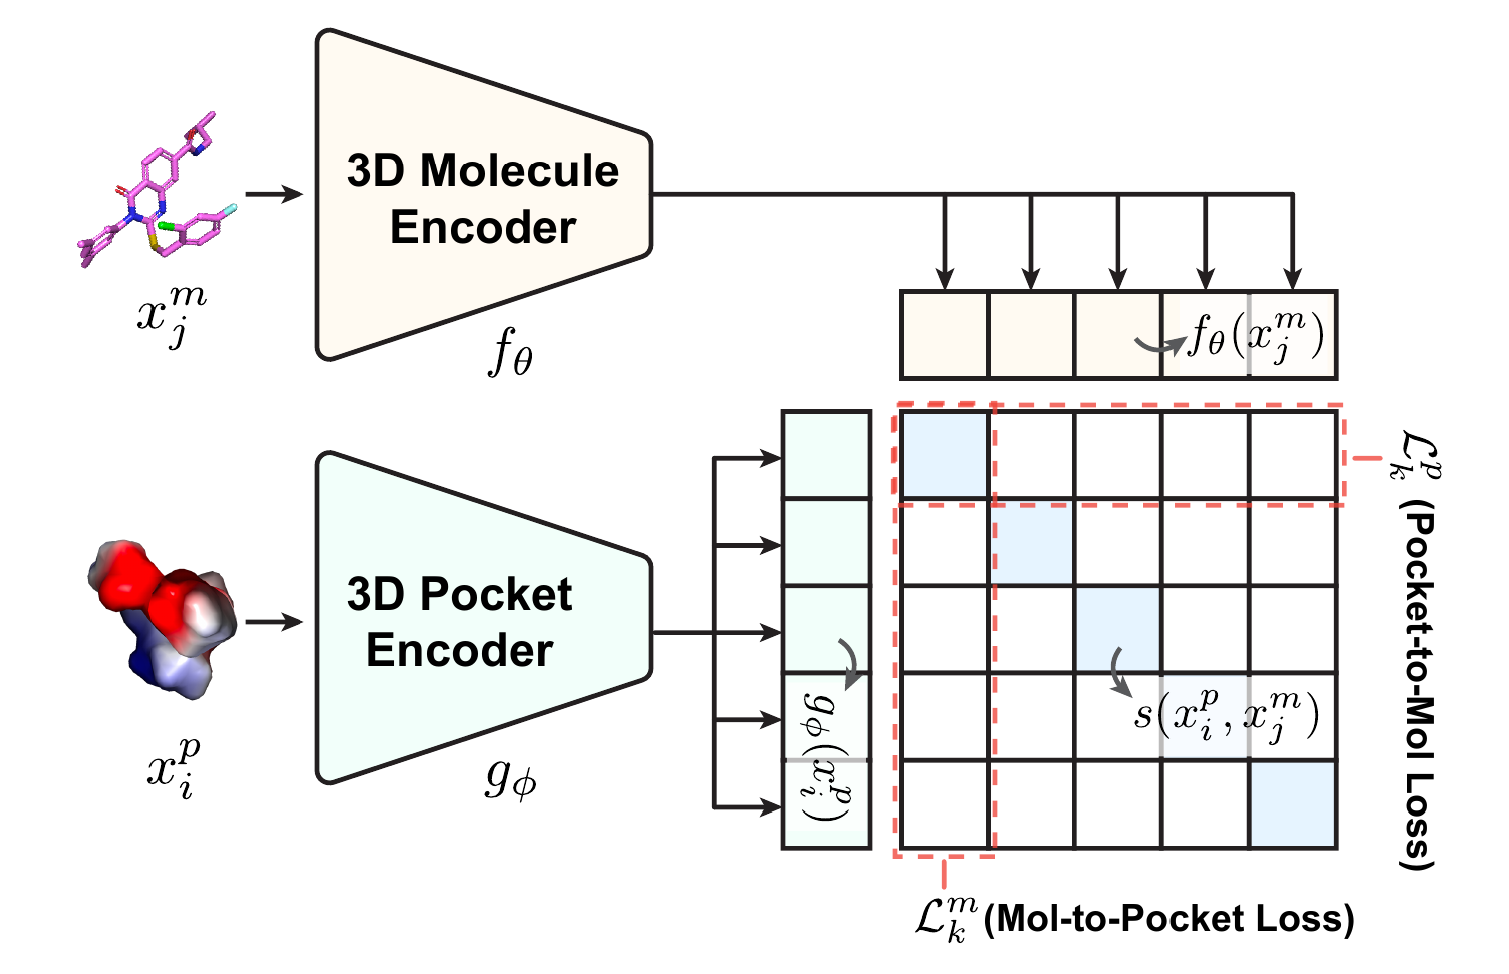
\includegraphics[width=.75\linewidth]{drugclip}

\caption{Overview of the DrugCLIP training process. Adapted from
  \citep{gao23:_drugc}.}
\label{fig:dc-training}
\end{figure}

Formally, the DrugCLIP loss function has two terms: in a batch of $N$
pairs, the \emph{pocket-to-mol loss} for pocket $x_k^p$ is defined as
\begin{equation}
  \label{eq:original-p2m-loss}
  \mathcal{L}_k^{p} (x_k^p, \{ x_i^m \}_{i=1}^N) =
  -\log
  \frac{
    \exp(s(x_k^p, x_k^m)/\tau)
  }{
    \sum_i \exp(s(x_k^p, x_i^m)/\tau)
  }
\end{equation}
and the \emph{mol-to-pocket loss} for molecule $x_k^m$ is defined as
\begin{equation}
  \label{eq:original-m2p-loss}
  \mathcal{L}_k^{m} = (x_k^m, \{ x_i^p \}_{i=1}^N) =
  -\log
  \frac{
    \exp(s(x_k^p, x_k^m)/\tau)
  }{
    \sum_i \exp(s(x_i^p, x_k^m)/\tau)
  }
\end{equation}
where $s(\cdot, \cdot)$ is defined in Eq.(\ref{eq:score}) and $\tau$
is a hyperparameter (called \emph{temperature}) that controls the
smoothness of the softmax distribution. The final loss for a batch
(which training seeks to minimize) is then
\begin{equation}
  \label{eq:original-loss}
  \mathcal{L} = 
  \frac{1}{2}
  \sum_{k=1}^N
  \left(
    \mathcal{L}_k^{p} + \mathcal{L}_k^{m}
  \right)
\end{equation}

The definitions above are important for the following section, where
we describe the modifications we applied to the training procedure in
order to fine-tune the model for the target-fishing problem.


\subsection{Fine-tuning formulation for target fishing}

\begin{itemize}
  \item Explain that the original DrugCLIP contrastive loss is naturally aligned with virtual screening, but not necessarily optimized for target fishing.

  \item Describe the issue with repeated ligands:
  \begin{itemize}
    \item the same molecule can appear in several positive protein-ligand complexes;
    \item those complexes may correspond to different structures, homologous proteins, isoforms, or related binding sites;
    \item in target fishing, all known pockets for the same molecule should be treated as positives;
    \item the original diagonal-only contrastive loss may treat some known positives as implicit negatives, depending on batch composition.
  \end{itemize}

  \item Define the set of known positive pockets for a molecule:
  \begin{equation}
  P^{+}(m) = \{p : (p,m) \in D\}
  \end{equation}

  \item Explain that \(D\) denotes the available set of observed positive pocket-molecule pairs.

  \item Define a positive-pair mask for a batch:
  \begin{equation}
  Y_{ij} =
  \begin{cases}
  1, & \text{if } p_j \in P^{+}(m_i)\\
  0, & \text{otherwise}
  \end{cases}
  \end{equation}

  \item Define the multi-positive molecule-to-pocket loss:
  \begin{equation}
  L^{m \rightarrow p}_{i}
  =
  - \log
  \frac{
    \sum_j Y_{ij} \exp(S_{ij}/\tau)
  }{
    \sum_j \exp(S_{ij}/\tau)
  }
  \end{equation}

  \item Explain that \(S_{ij}=s(p_j,m_i)\) is the similarity between pocket \(p_j\) and molecule \(m_i\), and that \(\tau\) is the contrastive temperature.

  \item Explain the intuition: for each query molecule, the loss increases the total softmax probability assigned to all known positive pockets in the batch.

  \item Present fine-tuning variants to be discussed:
  \begin{itemize}
    \item freeze both encoders and train only projection layers;
    \item train projection layers plus the temperature parameter;
    \item unfreeze upper encoder layers;
    \item train the full model with a smaller learning rate;
    \item compare molecule-to-pocket loss alone with a symmetric loss that also includes pocket-to-molecule terms.
  \end{itemize}

  \item State that the current implementation and experiments are preliminary and that the poor validation results do not yet support a performance claim.
\end{itemize}

\subsection{Benchmarking and diagnostic evaluation}

\begin{itemize}
  \item Explain that benchmarking target fishing is difficult because a query molecule may have several true targets, and missing pairs are not necessarily true negatives.

  \item Describe the implemented benchmark workflow:
  \begin{itemize}
    \item construct an explicit table of positive molecule-pocket pairs;
    \item build query-molecule LMDB files;
    \item build candidate-pocket LMDB files;
    \item run molecule-to-pocket retrieval;
    \item compare ranked lists against known positives;
    \item compute ranking metrics.
  \end{itemize}

  \item List metrics to be discussed:
  \begin{itemize}
    \item top-\(k\) accuracy;
    \item recall@\(k\);
    \item mean reciprocal rank;
    \item rank of the first known positive;
    \item enrichment-style metrics for early retrieval;
    \item AUROC only with caution, because it may be less informative when early ranking is the main objective.
  \end{itemize}

  \item Explain that preliminary results are poor for both the fine-tuned BioSensIA-DC model and the original DrugCLIP model in the current evaluation setup.

  \item Explain that this suggests the need for diagnostic work before any strong conclusion:
  \begin{itemize}
    \item verify data splits;
    \item verify checkpoint compatibility;
    \item verify LMDB contents;
    \item verify atom dictionaries;
    \item verify cached embeddings;
    \item verify whether candidate pockets match the positive-pair table;
    \item verify whether the benchmark task is consistent with the model's training assumptions.
  \end{itemize}
\end{itemize}

\subsection{Computational environment and reproducibility}

\begin{itemize}
  \item Describe the computational environment used for development:
  \begin{itemize}
    \item GNU/Linux;
    \item Python 3.11;
    \item PyTorch with CUDA;
    \item RDKit;
    \item Uni-Core;
    \item DrugCLIP;
    \item LMDB.
  \end{itemize}

  \item Explain the use of \texttt{uv} for Python environment management.

  \item Explain that a GPU is required by inherited constraints in the original DrugCLIP code path.

  \item Discuss technical issues encountered:
  \begin{itemize}
    \item compiling Uni-Core;
    \item CUDA extension compatibility;
    \item C++ standard-library compatibility;
    \item GPU memory limits;
    \item long-running embedding precomputation;
    \item embedding-cache invalidation.
  \end{itemize}

  \item Explain why these details matter: they affect reproducibility and practical adoption of 3D deep-learning models in computational biosensor research.
\end{itemize}


\section{RESULTS AND DISCUSSION}

\subsection{Implemented software artifacts}

\begin{itemize}
  \item Present the public repository as the main concrete result of this stage.

  \item List implemented artifacts:
  \begin{itemize}
    \item query-molecule LMDB generation;
    \item candidate-pocket LMDB generation;
    \item molecule-to-pocket retrieval;
    \item ranked-pocket output;
    \item preliminary benchmark code;
    \item installation and execution documentation.
  \end{itemize}

  \item Include a table with columns such as:
  \begin{itemize}
    \item file or module name;
    \item purpose;
    \item input;
    \item output;
    \item current status.
  \end{itemize}

  \item Discuss how these artifacts convert DrugCLIP from a virtual-screening-only workflow into a prototype that can also run target-fishing queries.
\end{itemize}

\subsection{Qualitative query example with okadaic acid}

\begin{itemize}
  \item Present okadaic acid as a qualitative sanity-check query.

  \item Explain the biological expectation: PP2A-related pockets should be considered relevant because PP2A is a known okadaic-acid target.

  \item Include a planned table with:
  \begin{itemize}
    \item rank;
    \item PDB identifier;
    \item score;
    \item protein or pocket annotation;
    \item whether the result is known, plausible, unclear, or likely irrelevant.
  \end{itemize}

  \item Discuss whether PP2A-associated structures appear near the top of the ranking.

  \item State clearly that this qualitative example is not a benchmark. It is only a sanity check and an illustration of the workflow.
\end{itemize}

\subsection{Preliminary quantitative results}

\begin{itemize}
  \item Report that the quantitative results obtained so far are unsatisfactory.

  \item Separate two observations:
  \begin{itemize}
    \item the fine-tuned BioSensIA-DC model currently performs poorly;
    \item the original DrugCLIP model also performs poorly under the current local benchmark workflow.
  \end{itemize}

  \item Avoid claiming improvement over DrugCLIP.

  \item Present the results as a diagnostic table, not as a final performance table. Suggested columns:
  \begin{itemize}
    \item model;
    \item checkpoint;
    \item query set;
    \item candidate-pocket set;
    \item metric values;
    \item diagnostic comment.
  \end{itemize}

  \item Explain that the current evidence points to unresolved issues in reproduction, data handling, benchmark construction, or model adaptation.
\end{itemize}

\subsection{Possible causes of the poor benchmark results}

\begin{itemize}
  \item Discuss possible data problems:
  \begin{itemize}
    \item mismatch between training, validation, and candidate LMDB files;
    \item differences between the downloaded data and the data used in the original DrugCLIP paper;
    \item duplicated PDB identifiers with different structures;
    \item ligand-identity inconsistencies;
    \item salt, tautomer, stereochemistry, or conformer inconsistencies.
  \end{itemize}

  \item Discuss possible implementation or protocol problems:
  \begin{itemize}
    \item wrong or incompatible checkpoint;
    \item stale cached embeddings;
    \item incorrect correspondence between pocket identifiers and benchmark positives;
    \item candidate libraries that do not contain the expected positives;
    \item metrics computed over an inappropriate candidate set;
    \item target-fishing evaluation derived from data originally organized for virtual screening.
  \end{itemize}

  \item Discuss possible modeling limitations:
  \begin{itemize}
    \item DrugCLIP was primarily motivated by virtual screening;
    \item target fishing is multi-positive by nature;
    \item unobserved pairs are not reliable true negatives;
    \item the similarity score is not physically calibrated;
    \item fine-tuning projection layers alone may be insufficient.
  \end{itemize}

  \item Conclude that the next step must be a systematic audit before interpreting the model's predictive value.
\end{itemize}

\subsection{Relationship to existing target-fishing tools}

\begin{itemize}
  \item Compare BioSensIA-DC conceptually with PharmMapper:
  \begin{itemize}
    \item PharmMapper performs reverse pharmacophore mapping;
    \item BioSensIA-DC performs learned molecule-pocket representation matching;
    \item both produce ranked target-candidate lists.
  \end{itemize}

  \item Compare BioSensIA-DC conceptually with SwissTargetPrediction:
  \begin{itemize}
    \item SwissTargetPrediction relies on similarity to known ligands;
    \item BioSensIA-DC relies on learned 3D compatibility between molecules and pockets;
    \item the two approaches may be complementary.
  \end{itemize}

  \item Discuss how future versions of BioSensIA could combine rankings from multiple methods:
  \begin{itemize}
    \item rank aggregation;
    \item consensus among tools;
    \item grouping by protein family;
    \item docking-based follow-up;
    \item literature-based validation.
  \end{itemize}
\end{itemize}

\subsection{Relevance to the BioSensIA project}

\begin{itemize}
  \item Explain that BioSensIA-DC is one module in a larger computational pipeline for biosensor-oriented bioreceptor discovery.

  \item Relate the prototype to planned BioSensIA components:
  \begin{itemize}
    \item UniProt and Gene Ontology queries;
    \item domain and family analysis;
    \item PDB and AlphaFold structural data;
    \item pocket prediction;
    \item docking and pharmacophore analysis;
    \item evidence aggregation for candidate bioreceptors.
  \end{itemize}

  \item Explain that even before full validation, BioSensIA-DC provides an operational way to turn a molecule-centered question into a ranked list of structural candidates.

  \item Emphasize that the current results motivate further validation rather than immediate deployment.
\end{itemize}


\section{CONCLUSIONS}

\subsection{Summary of contributions}

\begin{itemize}
  \item Summarize that the paper presented BioSensIA-DC, a DrugCLIP-based computational prototype for molecule-to-pocket target fishing.

  \item Highlight the main engineering contribution: implementing the reverse retrieval direction needed to rank candidate pockets for a query molecule.

  \item Highlight that the prototype includes data preparation, retrieval execution, ranked output generation, and preliminary evaluation tools.

  \item Highlight that the implementation is publicly available and intended to support reproducible development.
\end{itemize}

\subsection{Limitations}

\begin{itemize}
  \item State that the current model has not yet been validated as a reliable predictor.

  \item State that preliminary benchmark results are poor for both the fine-tuned model and the original DrugCLIP model in the current local evaluation setup.

  \item Explain that these results may reflect unresolved problems in reproduction, data consistency, benchmark construction, or the adaptation of DrugCLIP to target fishing.

  \item State that no claim of improved predictive performance is made in the present paper.
\end{itemize}

\subsection{Future work}

\begin{itemize}
  \item Reproduce the original DrugCLIP benchmarks more carefully before interpreting target-fishing results.

  \item Audit checkpoints, LMDB files, atom dictionaries, cached embeddings, and benchmark-positive definitions.

  \item Build a target-fishing benchmark with rigorous train-test separation and clear ligand-identity policies.

  \item Evaluate multi-conformer query strategies, including maximum, mean, median, quantile, and log-sum-exp aggregation.

  \item Expand the candidate-pocket library using PDB, BioLiP, sc-PDB, AlphaFold structures, and pocket-prediction tools.

  \item Compare BioSensIA-DC rankings with PharmMapper, SwissTargetPrediction, and docking-based validation.

  \item Integrate BioSensIA-DC into a broader BioSensIA interface for biosensor-oriented candidate discovery.
\end{itemize}


%%%%%%%%%%%%%%%%%%%%%%%%%%%%%%%%%%%%%%%%%%%%%%%%%%%%%%%%%%%%%%%%%%%%%
% Acknowledgements and AI disclosure
%%%%%%%%%%%%%%%%%%%%%%%%%%%%%%%%%%%%%%%%%%%%%%%%%%%%%%%%%%%%%%%%%%%%%

\section*{Acknowledgements}

\begin{itemize}
  \item Acknowledge computational infrastructure, collaborators, and funding sources, if applicable.

  \item Include the required generative-AI disclosure. Suggested wording:
  \begin{itemize}
    \item The author used ChatGPT (OpenAI) to assist with manuscript organization, language revision, and discussion of alternative formulations. All scientific content, interpretation of results, and conclusions remain the responsibility of the author.
  \end{itemize}
\end{itemize}

% (todo o restante do conteúdo do template permanece exatamente igual)

\bibliographystyle{apalike}
\fontsize{11}{0}\selectfont
\bibliography{bib/references}


\end{document}
%%% Local Variables:
%%% mode: LaTeX
%%% TeX-master: t
%%% End:
